%% fancy header & foot
\pagestyle{fancy}
\lhead{[ELEC-H-2001] Électricité\\ TP \no 3 : Circuits linéaires et permanents avec source sinusoïdale\ifthenelse{\boolean{corrige}}{~-- corrigé}{}}
\rhead{v1.0.1\\ page \thepage}
\cfoot{}
%%

\pdfinfo{
/Author (Raoul Sommeillier, ULB -- BEAMS)
/Title (TP 3 ELEC-H-2001, Circuits linéaires et permanents soumis à une sollicitation sinusoïdale)
/ModDate (D:\pdfdate)
}

\hypersetup{
pdftitle={TP 3 [ELEC-H-2001] Électricité : Circuits linéaires et permanents soumis à une sollicitation sinusoïdale},
pdfauthor={Raoul Sommeillier, ©2018 ULB - BEAMS  },
%pdfsubject={filtrage et analyse fréquentielle}
}

%\date{\vspace{-1cm}\mydate\today}
%\title{\vspace{-2cm} Labo \no 6\\ Électronique appliquée [ELEC-H-301]\\Réalisation d'un ampli à transistor\ifthenelse{\boolean{corrige}}{~\\Corrigé}{}}

%\author{\vspace{-1cm}}%\textsc{Yannick Allard}}

\setlength{\parskip}{0.5cm plus4mm minus3mm} %espacement entre §
\setlength{\parindent}{0pt}


\begin{document}

\tptitle{}{Séance 3~: Circuits linéaires et permanents soumis à une sollicitation sinusoïdale}

\section{Pré-requis}
Avant la séance, vous aurez lu attentivement l'énoncé de la manipulation. Vous aurez par ailleurs relu les chapitres et sections suivants:

\begin{itemize}
	\item Chapitre 5 - Résoudre un circuit : procédure de base et accélérateur
	\begin{itemize}
		\item Section 5.1 - Vocabulaire lié aux circuits
		\begin{itemize}
			\item 5.1.2 Connexions série et parallèle 
			\item 5.1.3 Branche
			\item 5.1.4 Maille 
		\end{itemize}
		\item Section 5.2 - Lois de Kirchhoff
	\end{itemize}
	\item Chapitre 6 - Résoudre un circuit réactif dans le domaine temporel
	\begin{itemize}
		\item Section 6.5 - Analyse temporelle du circuit RL (source sinusoïdale)
		\item Section 6.6 - Analyse temporelle du circuit RLC
	\end{itemize}
	\item Chapitre 7 - Résoudre un circuit réactif dans le domaine fréquentiel
	\begin{itemize}
		\item Section 7.3 - Phaseur
		\item Section 7.4 - Impédances et admittances
		\begin{itemize}
			\item 7.4.2 Impédance d'une capacité pure
			\item 7.4.3 Impédance d'une résistance pure 
		\end{itemize}
	\end{itemize}

\end{itemize}

\vspace{5pt}

\newpage


\section{Exercices}
\subsection{RL}
La tension $e(t)=V_m \cos(\omega t+\alpha)$ est appliquée à l'instant $t=t_0=0$ au circuit $RL$.
\begin{center}
\begin{circuitikz} \draw
(0,0)	to[sinusoidal voltage source, v=$e(t)$, i^>=$i$]		(0,4)
		to[closing switch, l=$t_0$]		(3,4)
		to[R, l=$R$]					(3,2)
		to[L, l=$L$]					(3,0)--(0,0)
;
\end{circuitikz}
\end{center}

\Question
{%Q
\textit{Déterminer l'expression du courant $i(t)$ pour tout temps $t$ et discuter la valeur de $\alpha$ pour que:
\begin{enumerate}
\item le régime permanent s'établisse immédiatement
\item la valeur instantanée du courant soit maximale
\end{enumerate}}
}
{%C
La solution générale est (cfr cours):
$$i(t)=i'(t)+i''(t)=I_m \cos(\omega t + \alpha -\theta) - I_m \cos(\alpha -\theta) e^{-t/\tau}$$
Où $i'(t)$ est le terme de régime et $i''(t)$ le terme transitoire.

$$I_m=\frac{V_m}{\sqrt{{R^2}+(\omega L)^2}}$$
$$tan(\theta)=\frac{\omega L}{R}$$
$$\tau=\frac{L}{R}$$

Le transitoire est nul si $\cos(\alpha -\theta)=0 \Leftrightarrow \alpha -\theta=\pm \pi/2$.\\
Cela correspond à un enclenchement du circuit ($t=0$) au moment où le terme de régime passe par zéro. Dans ce cas, le régime permanent s'établit immédiatement.\\

Le terme transitoire sera maximum lorsque le circuit est enclenché au moment où le terme de régime passe par son maximum positif ou négatif ($\pm I_m$).
$$\alpha - \theta =0 \ ou \ \pi \Leftrightarrow i(t)=\pm I_m (\cos(\omega t) - e^{-\frac{R}{L}t})$$

Si $\omega L >> R$, le terme transitoire garde une valeur appréciable pendant plusieurs périodes.\\
Dans ce cas, le courant total atteint sa valeur maximale $i_{max}$ environ une demi-période après le branchement, lorsque le terme de régime s'approche de sa valeur maximale, mais a le même signe que le terme transitoire:
$$i_{max}=i(T/2)\simeq I_m (1+e^{-\frac{R}{L}\frac{T}{2}})=I_m (1+e^{-\pi \frac{R}{\omega L}}) \simeq 2I_m \ (si \frac{R}{\omega L}\ est\ petit)$$
\begin{center}
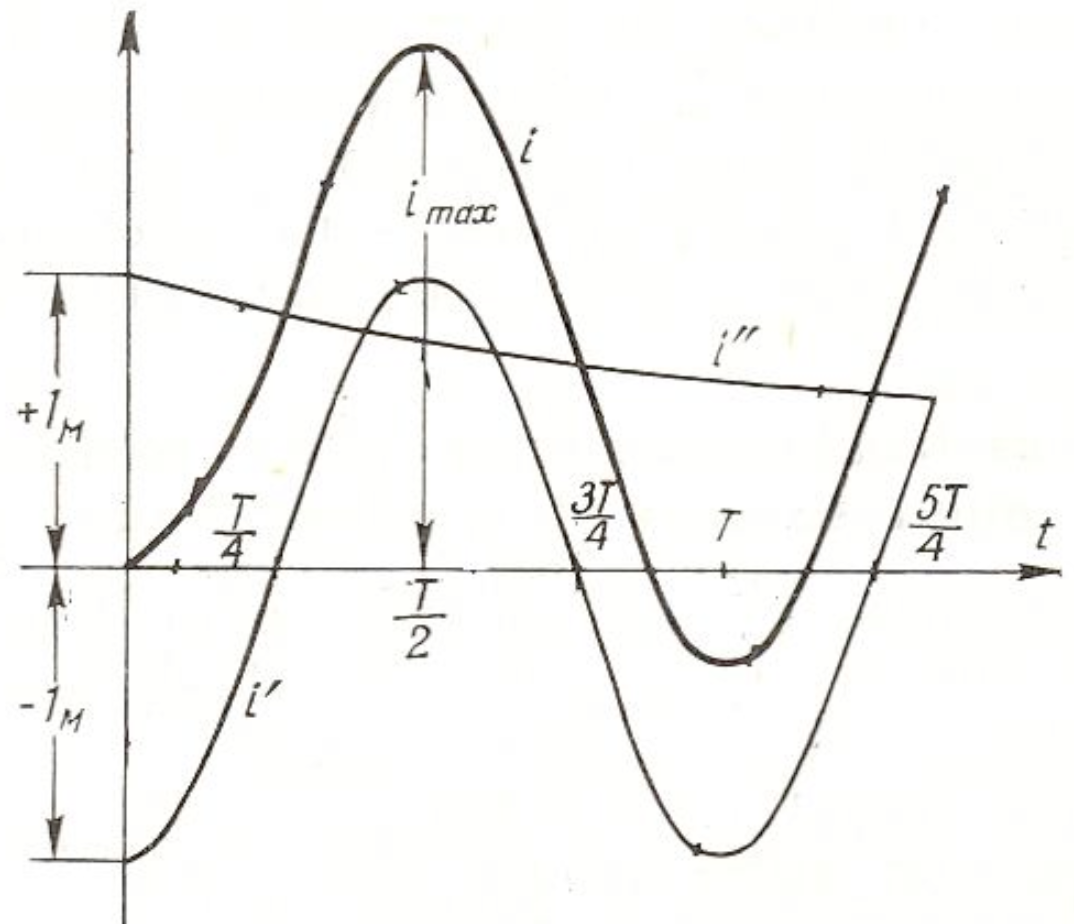
\includegraphics[scale=0.3]{TP3/TP3-Exo1.PNG}
\end{center}
}
{}


\subsection{Résoudre le circuit}
Pour le circuit suivant
\begin{center}
\begin{circuitikz} \draw
(0,0)	to[sinusoidal voltage source, v=$v_g(t)$]		(0,4)
		to[R, l=$R_1$]					(2,4)
		to[short]           (4,4)
(0,0)--(4,0)
		to[C, l=$C$, v>=$v_C(t)$]		(4,4)
(2,4)	to[R, l=$R_2$]					(2,2)
		to[L, l=$L$]					(2,0)
;
\end{circuitikz}
\end{center}
Où $v_g(t)=\sin (4t + 45^o)$, $R_1=4\Omega$, $R_2=1\Omega$, $L=1H$ et $C=\frac{1}{4}F$.

\Question
{%Q
\textit{Déterminer la tension aux bornes de la capacité en régime.}
}
{%C
\begin{center}
\begin{circuitikz} \draw
(0,0)	to[sinusoidal voltage source, v=$v_g(t)$, i^>=$i_g(t)$]		(0,4)
		to[R, l=$R_1$]					(2,4)
		to[short, i=$i_C(t)$]           (4,4)
(0,0)--(4,0)
		to[C, l=$C$, v>=$v_C(t)$]		(4,4)
(2,4)	to[R, l=$R_2$, i=$i_L(t)$]					(2,2)
		to[L, l=$L$]					(2,0)
;
\end{circuitikz}
\end{center}
Ayant défini les grandeurs dans le schéma, les lois des mailles, des noeuds et des composants permettent d'écrire:\\
$\underline{V}_g=R_1\underline{I}+\underline{V}_C=R_1(\underline{I}_L+\underline{I}_C)+\underline{V}_C$\\
$(R_2+j\omega L)\underline{I}_L=\underline{V}_C$\\
$\underline{V}_C=\frac{\underline{I}_C}{j\omega C}$

$\Rightarrow \underline{V}_C=\underline{V}_g \frac{R_2+j\omega L}{R_1(1-\omega^2LC)+R_2+j(\omega L+\omega CR_1R_2)}$

$\underline{V}_g=e^{j45^o}$ (avec des phaseurs en sinus comme dans l'énoncé, sinon déphaser de $90^o$)\\
$\Rightarrow \underline{V}_C=e^{j45^o}\frac{1+j4}{-11+j8}=e^{j45^o}\frac{4,12e^{j75,96^o}}{13,6e^{j143,97^o}}=0,303e^{-j23^o}$

L'expression finale en temporel est donc:\\ 
$v_C(t)=0,303 \sin(4t-23^o)$
}
{%A
}


\subsection{Résoudre le circuit 2}
Le circuit suivant se trouve en régime avant l'instant $t=t_0=0$ de fermeture de l'interrupteur. 
\begin{center}
\begin{circuitikz} \draw
(0,0)	to[sinusoidal voltage source, l=$e(t)$]		(0,2)
		to[R, l=$R_1$]								(2,2)
		to[closing switch, l=$t_0$]					(4,2)
		to[R, l=$R_2$]								(4,0)--(0,0)
(2,2)	to[C, l=$C$]								(2,0)
;
\end{circuitikz}
\end{center}
\Question
{%Q
\textit{Déterminer les courants pour toute valeur de $t$, avec $e(t)=E_0 \cos(\omega t)$.}
}
{%C
\begin{center}
\begin{circuitikz} \draw
(0,0)	to[sinusoidal voltage source, l=$e(t)$]		(0,2)
		to[R, l=$R_1$, i=$i_0$]								(2,2)
		to[closing switch, l=$t_0$]					(4,2)
		to[R, l=$R_2$, i=$i_2$]								(4,0)--(0,0)
(2,2)	to[C, l=$C$, i=$i_1$]								(2,0)
;
\end{circuitikz}
\end{center}

\begin{itemize}
\item \textbf{Pour $t<0$ (état de régime)}\\
$i_1(t)=i_0(t)$ et $i_2(t)=0$

$\underline{I}_0=\frac{E_0}{R_1+\frac{1}{j\omega C}}=\frac{j\omega CE_0}{1+j\omega CR_1}$\\
$\Rightarrow i_0(t)=\frac{\omega CE_0}{\sqrt{1+\omega^2 C^2 R_1^2}}\cos(\omega t+\phi)$ avec $tan(\phi)=\frac{1}{\omega CR_1}$\\

$\underline{V}_C=\frac{\underline{I}_0}{j\omega C}=\frac{E_0}{1+j\omega CR_1}$\\
$\Rightarrow v_C(t)=\frac{E_0}{\sqrt{1+\omega^2 C^2 R_1^2}}\cos(\omega t-\alpha)$ et $tan(\alpha)=\omega CR_1$
\item \textbf{Pour $t>0$}\\
$E_0 \cos(\omega t)=R_1(i_1+i_2)+R_2i_2$ \hspace{1cm}$(1)$\\
$v_C(0)+\frac{1}{C}\int_0^t i_1(\xi)d\xi=R_2i_2 \Rightarrow i_1=CR_2\frac{di_2}{dt}$\hspace{1cm}$(2)$\\
$(1)$ et $(2)$ $\Rightarrow E_0 \cos(\omega t)=(R_1+R_2)i_2+CR_1R_2\frac{di_2}{dt}$\\
$\Rightarrow i_2(t)=Ae^{-t\frac{R_1+R_2}{CR_1R_2}}+sol.\ partic.$\\

Pour chercher la solution particulière en $t>0$, $i_{2_p}(t)$, on va utiliser la méthode des phaseurs:\\
$\frac{1}{j\omega C}\underline{I}_1=R_2\underline{I}_2$\\
$\underline{E}_0=R_1(\underline{I}_1+\underline{I}_2)+R_2\underline{I}_2$\\

$\Rightarrow \underline{I}_2=\frac{E_0}{R_1+R_2+j\omega CR_1R_2}$\\
$\underline{I}_1=\frac{j\omega CR_2E_0}{R_1+R_2+j \omega CR_1R_2}$\\

La solution particulière est donc:\\
$$i_{2_p}(t)=K \cos(\omega t-\beta)$$
où $K=\frac{E_0}{\sqrt{(R_1+R_2)^2+(\omega CR_1R_2)^2}}$, $tan(\beta)=\omega \tau$ et $\tau=\frac{R_1R_2C}{R_1+R_2}$\\

La solution générale pour $t>0$ est alors:\\
$i_2(t)=Ae^{-t/\tau}+K \cos(\omega t-\beta)$\\
et il faut identifier $A$ à partir de la condition initiale.\\

\item \textbf{Condition initiale ($t=0^+$)}\\
$i_2(0^+)=\frac{v_C(0^+)}{R_2}=\frac{v_C(0^-)}{R_2}=\frac{E_0 \cos(\alpha)}{R_2\sqrt{1+\omega^2 C^2 R_1^2}}$\\
$A=\frac{E_0 \cos(\alpha)}{R_2\sqrt{1+\omega^2 C^2 R_1^2}}-K\cos(\beta)$\\

On a $i_2(t)$ pour $t>0$ (ouf!):\\
$i_2(t)=Ae^{-t/\tau}+K \cos(\omega t-\beta)$\\
$i_2(t)=\frac{E_0 \cos(\alpha)}{R_2\sqrt{1+\omega^2 C^2 R_1^2}}-K\cos(\beta)e^{-t\frac{R_1+R_2}{R_1R_2C}}+\frac{E_0}{\sqrt{(R_1+R_2)^2+(\omega CR_1R_2)^2}}\cos(\omega t-\beta)$

\item \textbf{Pour les autres courants en $t>0$}\\
$i_1(t)=CR_2\frac{di_2}{dt}=-\frac{CR_2}{\tau}Ae^{-t/\tau}-KCR_2\omega \sin(\omega t-\beta)$\\
$i_0(t)=i_1(t)+i_2(t)$
\end{itemize}
}
{%A
}


\subsection{Oscilloscope}
Le signal $V_e$ à mesurer est connecté à un oscilloscope au moyen d'une sonde externe. La sonde est constituée d'une résistance $R_S$ et d'une capacité $C_P$ (réglable) en parallèle.\\
L'impédance d'entrée de l'oscilloscope est modélisée par la mise en parallèle de $R_{in}=1M\Omega$ et $C_{in}=20pF$.\\
 
\begin{center}
\begin{circuitikz} \draw
node[ocirc] (A) at (0,2) {}
node[ocirc] (B) at (0,0) {}
(B) to [open, v^=$V_e$] (A)
node[ocirc] (C) at (3.5,2) {}
node[ocirc] (D) at (3.5,0) {}
(D) to [open, v^=$V_{in}$] (C)
(0,2)--(1,2)
		to[R, l=$R_S$]		(3,2)--(7,2)
		to[C, l=$C_{in}$]	(7,0)
(5,2)	to[R, l=$R_{in}$]	(5,0)
(1,2)--(1,3.5)
		to[variable capacitor, l=$C_P$, mirror]	(3,3.5)--(3,2)
(0,0)--(5,0)	
(5,0) node[ground] {}
(7,0) node[ground] {}
node[]() at (6.25,4){Oscilloscope}
;
\draw[dashed](4,-1)--(4,5)--(8.5,5)--(8.5,-1)--(4,-1);
\end{circuitikz}
\end{center}
\Question
{%Q
\textit{Déterminer les éléments de la sonde pour réaliser un facteur de division de $k$ (par exemple $k=10$) sans déformer le signal mesuré.\\
Dans ces conditions, déterminer la nouvelle impédance d'entrée équivalente.}
}
{%C
La sonde (externe) à haute impédance permet de connecter le signal à étudier à l'oscilloscope tout en réalisant un facteur de division (par exemple 10 ou 100) indépendant de la fréquence.\\
La sonde est constituée d'une résistance $R_S$ fixe et d'un condensateur $C_P$ réglable.\\

Le rapport de division est:\\
$$\frac{\underline{V}_{in}}{\underline{V}_e}=\frac{Z_{in}}{Z_S+Z_{in}}=\frac{1}{1+\frac{R_S}{R_{in}}\frac{1+j\omega R_{in}C_{in}}{1+j\omega R_{S}C_{P}}}$$

Pour que le signal à l'entrée de l'oscilloscope ne soit pas déformé, il faut que ce rapport soit indépendant de la fréquence (la sonde sera alors dite \underline{adaptée}):\\
$$R_SC_P=R_{in}C_{in} \hspace{1cm} (1)$$

Le rapport $\frac{1}{k}=\frac{\underline{V}_{in}}{\underline{V}_e}=\frac{R_{in}}{R_S+R_{in}}$ sera réel et indépendant de $\omega$. On aura donc:\\
$$R_S=(k-1)R_{in} \ et \ C_P=\frac{C_{in}}{k-1}$$
où $k$ est le \underline{rapport d'atténuation} de la sonde.\\

Exemple: $R_{in}=1M\Omega$, $C_{in}=20pF$, $k=10$ $\Rightarrow R_S=9M\Omega$ et $C_P=2,2pF$\\

Si la condition d'adaptation $(1)$ de la sonde est réalisée, l'impédance d'entrée de l'oscilloscope muni de la sonde est:\\
$$Z_e=Z_{in}+Z_S=\frac{R_{in}}{1+j\omega R_{in}C_{in}}+\frac{R_{S}}{1+j\omega R_{S}C_{P}}=\frac{R_{in}+R_S}{1+j\omega (R_{in}+R_S) \frac{C_{in}C_P}{C_{in}+C_P}}$$

La résistance d'entrée et la capacité d'entrée sont devenues:\\
$$R_e=R_{in}+R_S=kR_{in}$$
$$C_e=\frac{C_{in}C_P}{C_{in}+C_P}=\frac{C_{in}}{k}$$\\

La sonde permet donc d'augmenter la résistance d'entrée et de diminuer la capacité d'entrée.\\

Pour l'exemple: $R_e=10M\Omega$ et $C_e=2pF$.
}
{}

\subsection{RLC}
Pour le circuit RLC série en régime sinusoïdal permanent suivant:
\begin{center}
\begin{circuitikz} \draw
(0,0)	to[sinusoidal voltage source, v=$V_g$]		(0,3)
		to[R, l=$R$, v<=$V_R$]		(3,3)
		to[L, l=$L$, v<=$V_L$]		(6,3)
		to[C, l=$C$, v<=$V_C$]		(6,0)--(0,0)
;
\end{circuitikz}
\end{center}
\Question
{%Q
\textit{Représenter les phaseurs des différentes tensions dans le plan complexe (diagramme des phaseurs), en prenant le courant comme origine des phases. On se placera successivement dans le cas $\omega > \omega_0$, $\omega < \omega_0$, $\omega = \omega_0$, avec $\omega = \frac{1}{LC}$.}
}
{%C
$\underline{V}_g=\underline{V}_R+\underline{V}_L+\underline{V}_C$\\
$\underline{V}_R=R\underline{I}$\\
$\underline{V}_L=j\omega L\underline{I}$\\
$\underline{V}_C=-j\frac{1}{\omega C}\underline{I}$
$$\Rightarrow \underline{I}=\frac{\underline{V}_g}{Z}=\frac{\underline{V}_g}{R+j(\omega L-\frac{1}{\omega C})}$$

\begin{itemize}
\item $\omega>\omega_0 \Rightarrow |\underline{V}_L|>|\underline{V}_C|$\\
Le circuit est globalement inductif et le courant est en retard (de $\theta$) sur la tension.
\item $\omega<\omega_0 \Rightarrow |\underline{V}_L|<|\underline{V}_C|$\\
Le circuit est globalement capacitif et le courant est en avance sur la tension.
\item $\omega=\omega_0 \Rightarrow |\underline{V}_L|=|\underline{V}_C|$\\
Les réactances inductive et capacitive se compensent exactement. Le courant et la tension sont en phase.
\end{itemize}
\begin{center}
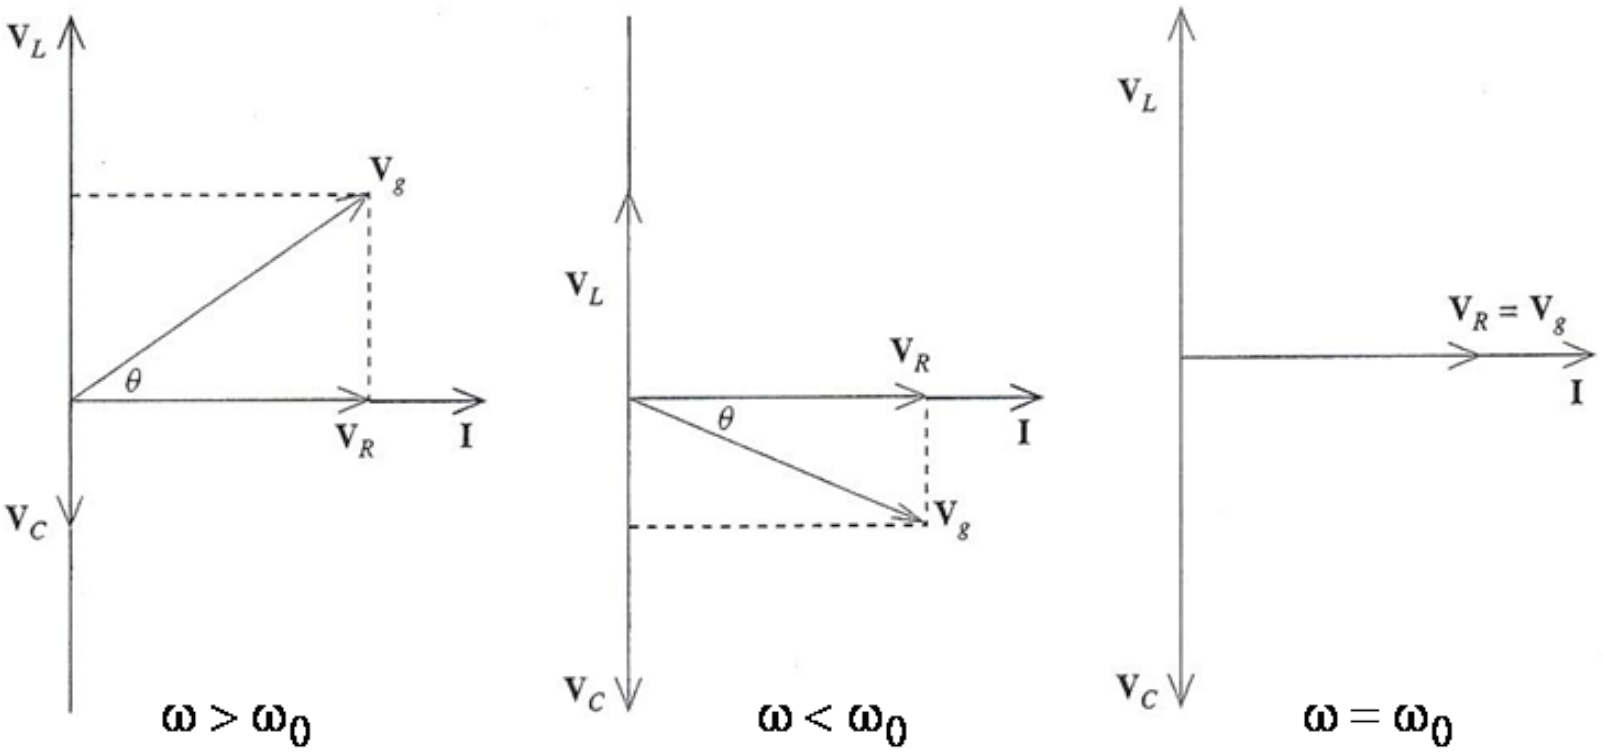
\includegraphics[scale=0.3]{TP3/TP3-Exo5.PNG}
\end{center}
}{}

\Question
{%Q
\textit{La tension $V_C$ peut-elle devenir supérieure à la tension d'alimentation?}
}
{%C
Affirmatif, c'est le principe de la résonance.\\
$V_C$ (et $V_L$) peuvent devenir supérieures à $V_g$. Par contre, $V_R$ ne peut pas dépasser $V_g$.
}



\end{document}